\documentclass[t, xcolor={dvipsnames}]{beamer}

\usepackage{amsmath}
\usepackage{tipa}
\usepackage{eso-pic}
\usepackage{graphicx}
\usepackage{svg}
\usepackage{listings}
\usepackage{wrapfig}
\usepackage{scrextend}
\usepackage{subfig}
\usepackage[export]{adjustbox}
\usepackage{apacite}
\bibliographystyle{apacite}
\renewcommand\bibliographytypesize{\tiny}


\setsvg{svgpath = img/}

\makeatletter
  \newenvironment{withoutheadline}{%
    \setbeamertemplate{headline}[default]
    \def\beamer@entrycode{\vspace*{-\headheight}}
    \setbeamertemplate{footline}[default]
  }{}
\makeatother

\usetheme{Malmoe}
\usecolortheme{dolphin}
\setbeamercolor{structure}{bg=red}

\title{\vspace{0.8cm}Automatic Birdsong Recognition}
\author{Victor F. L. Rodrigues}
\institute{School of Computer Science\\ The University of Manchester}
\titlegraphic{\includesvg[height=15mm]{UniOfManchesterLogo}}
\logo{\includesvg[height=4mm]{UniOfManchesterLogo}}

\begin{document}

%\usebackgroundtemplate{%
%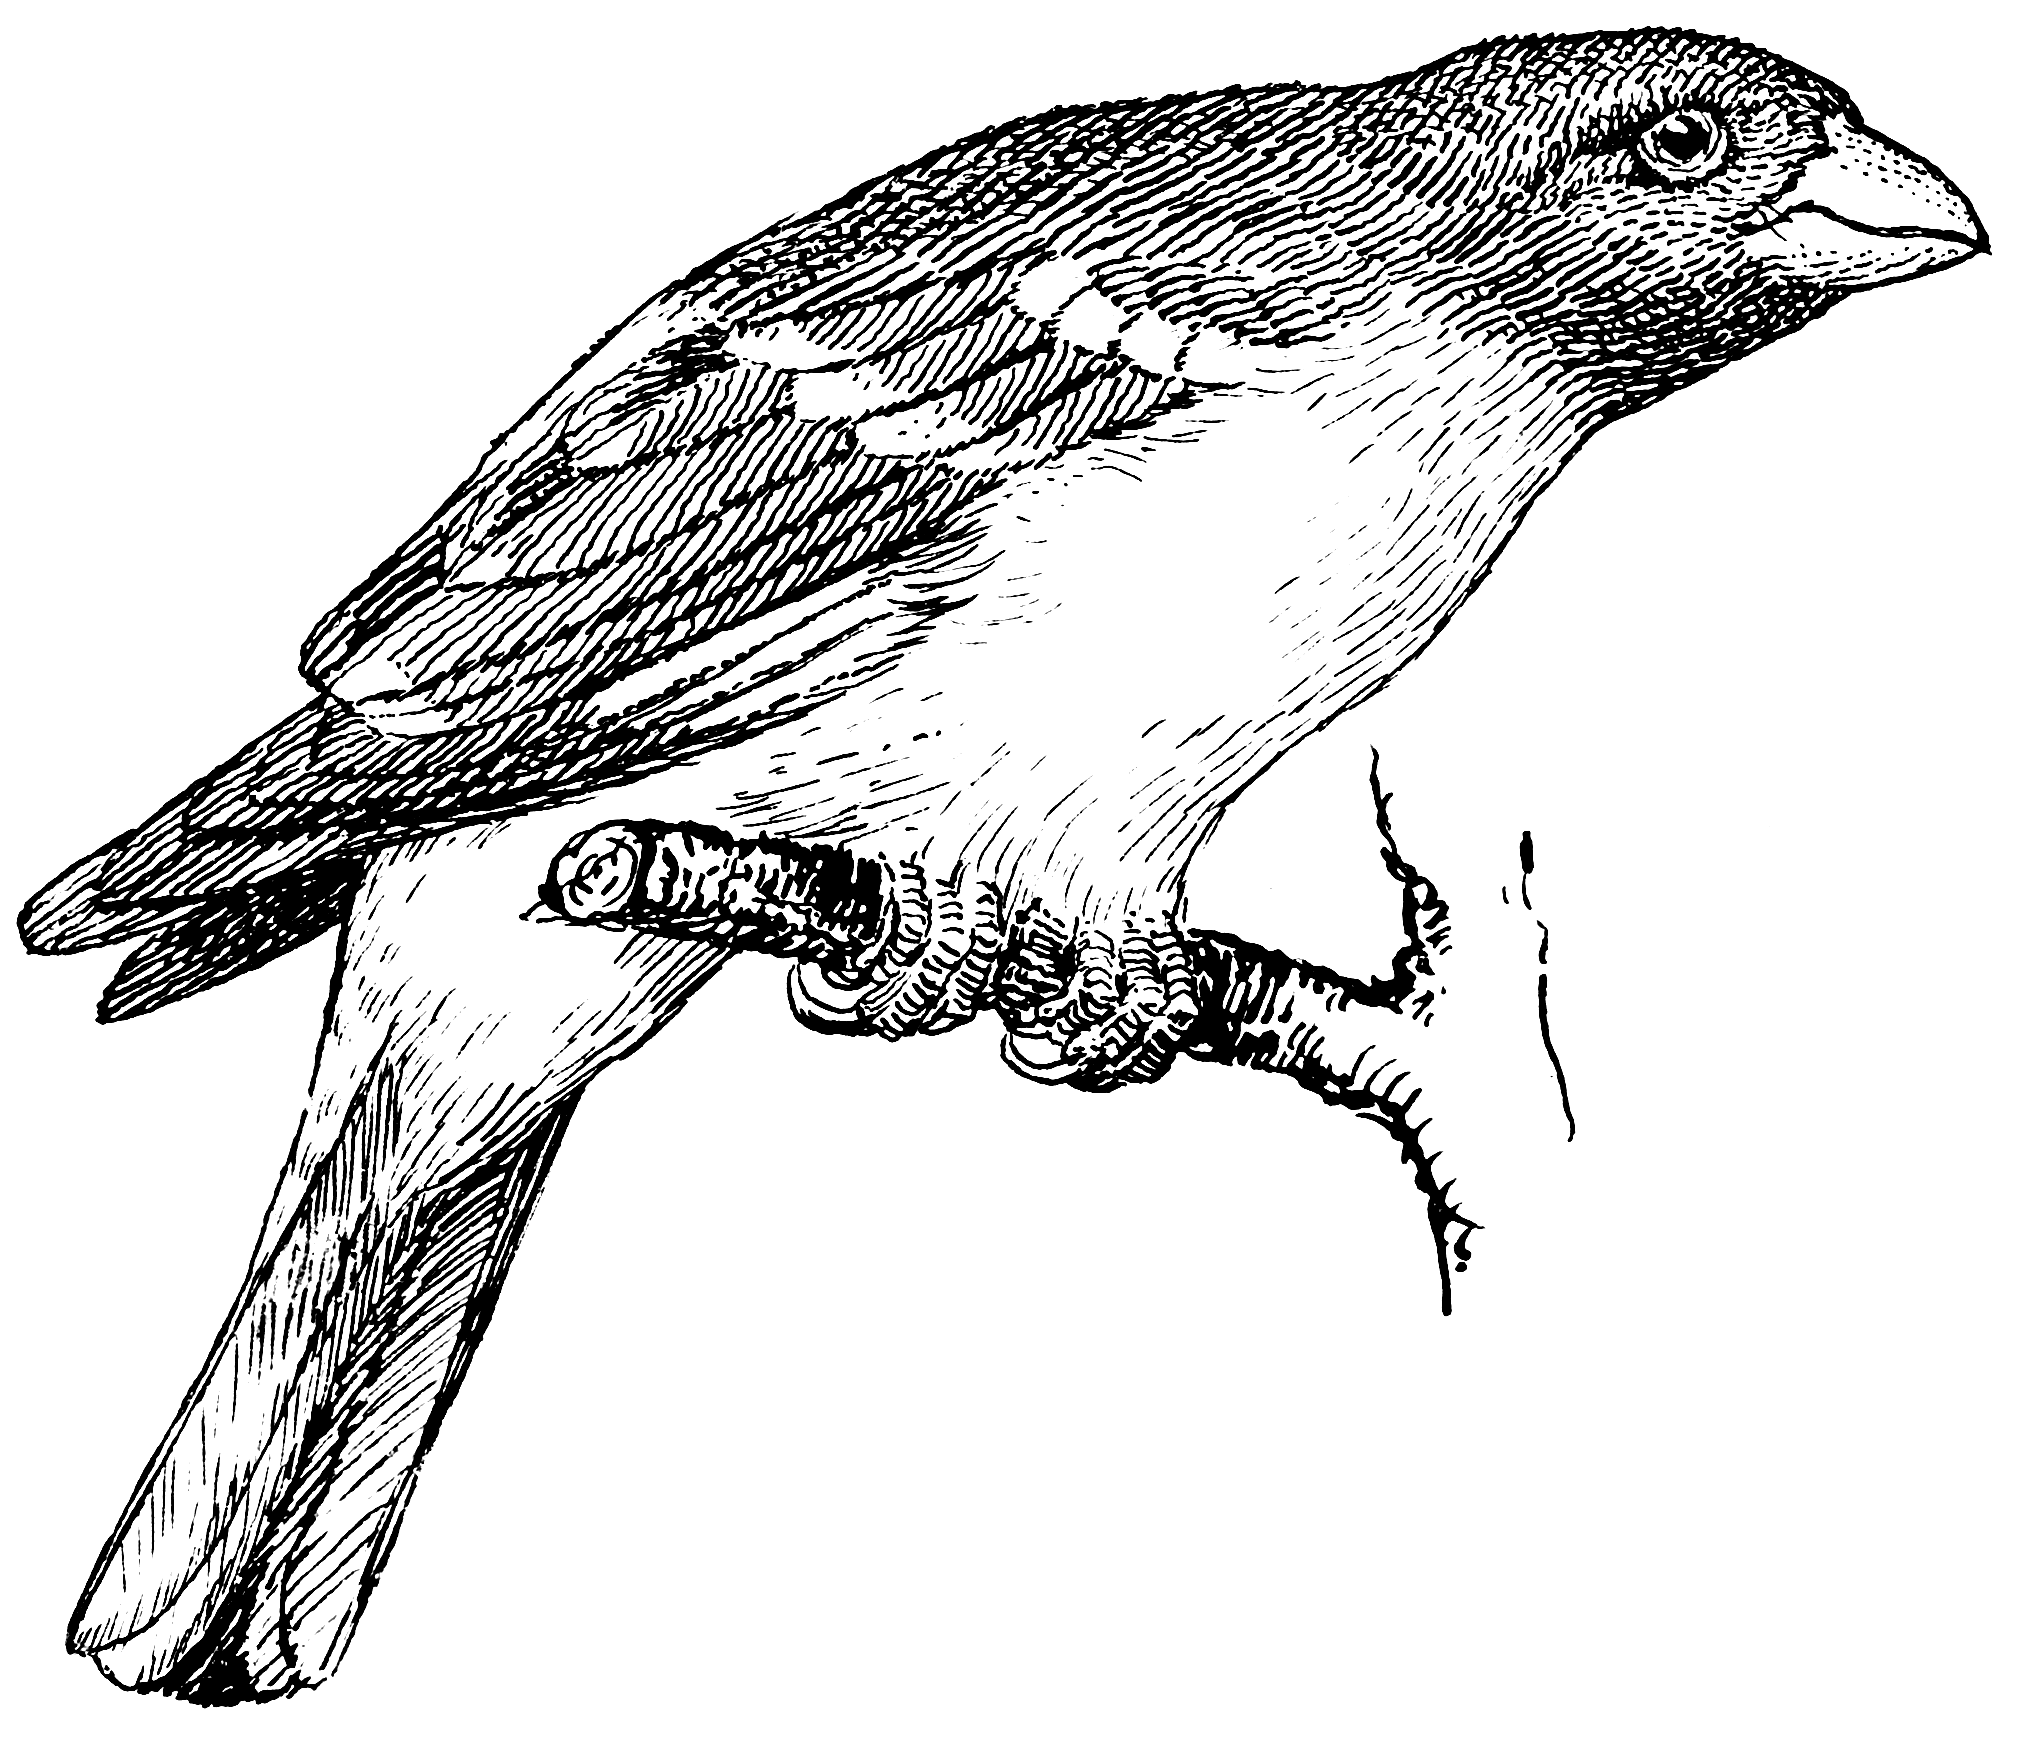
\includegraphics[width=0.5\paperwidth,height=0.5\paperheight,keepaspectratio=true]{img/Grossbeak_(PSF).png}
%}

\begin{withoutheadline}
  \begin{frame}[plain]
    \begin{wrapfigure}{L}[20cm]{0.23\textwidth}
      \vspace{0.2cm}
  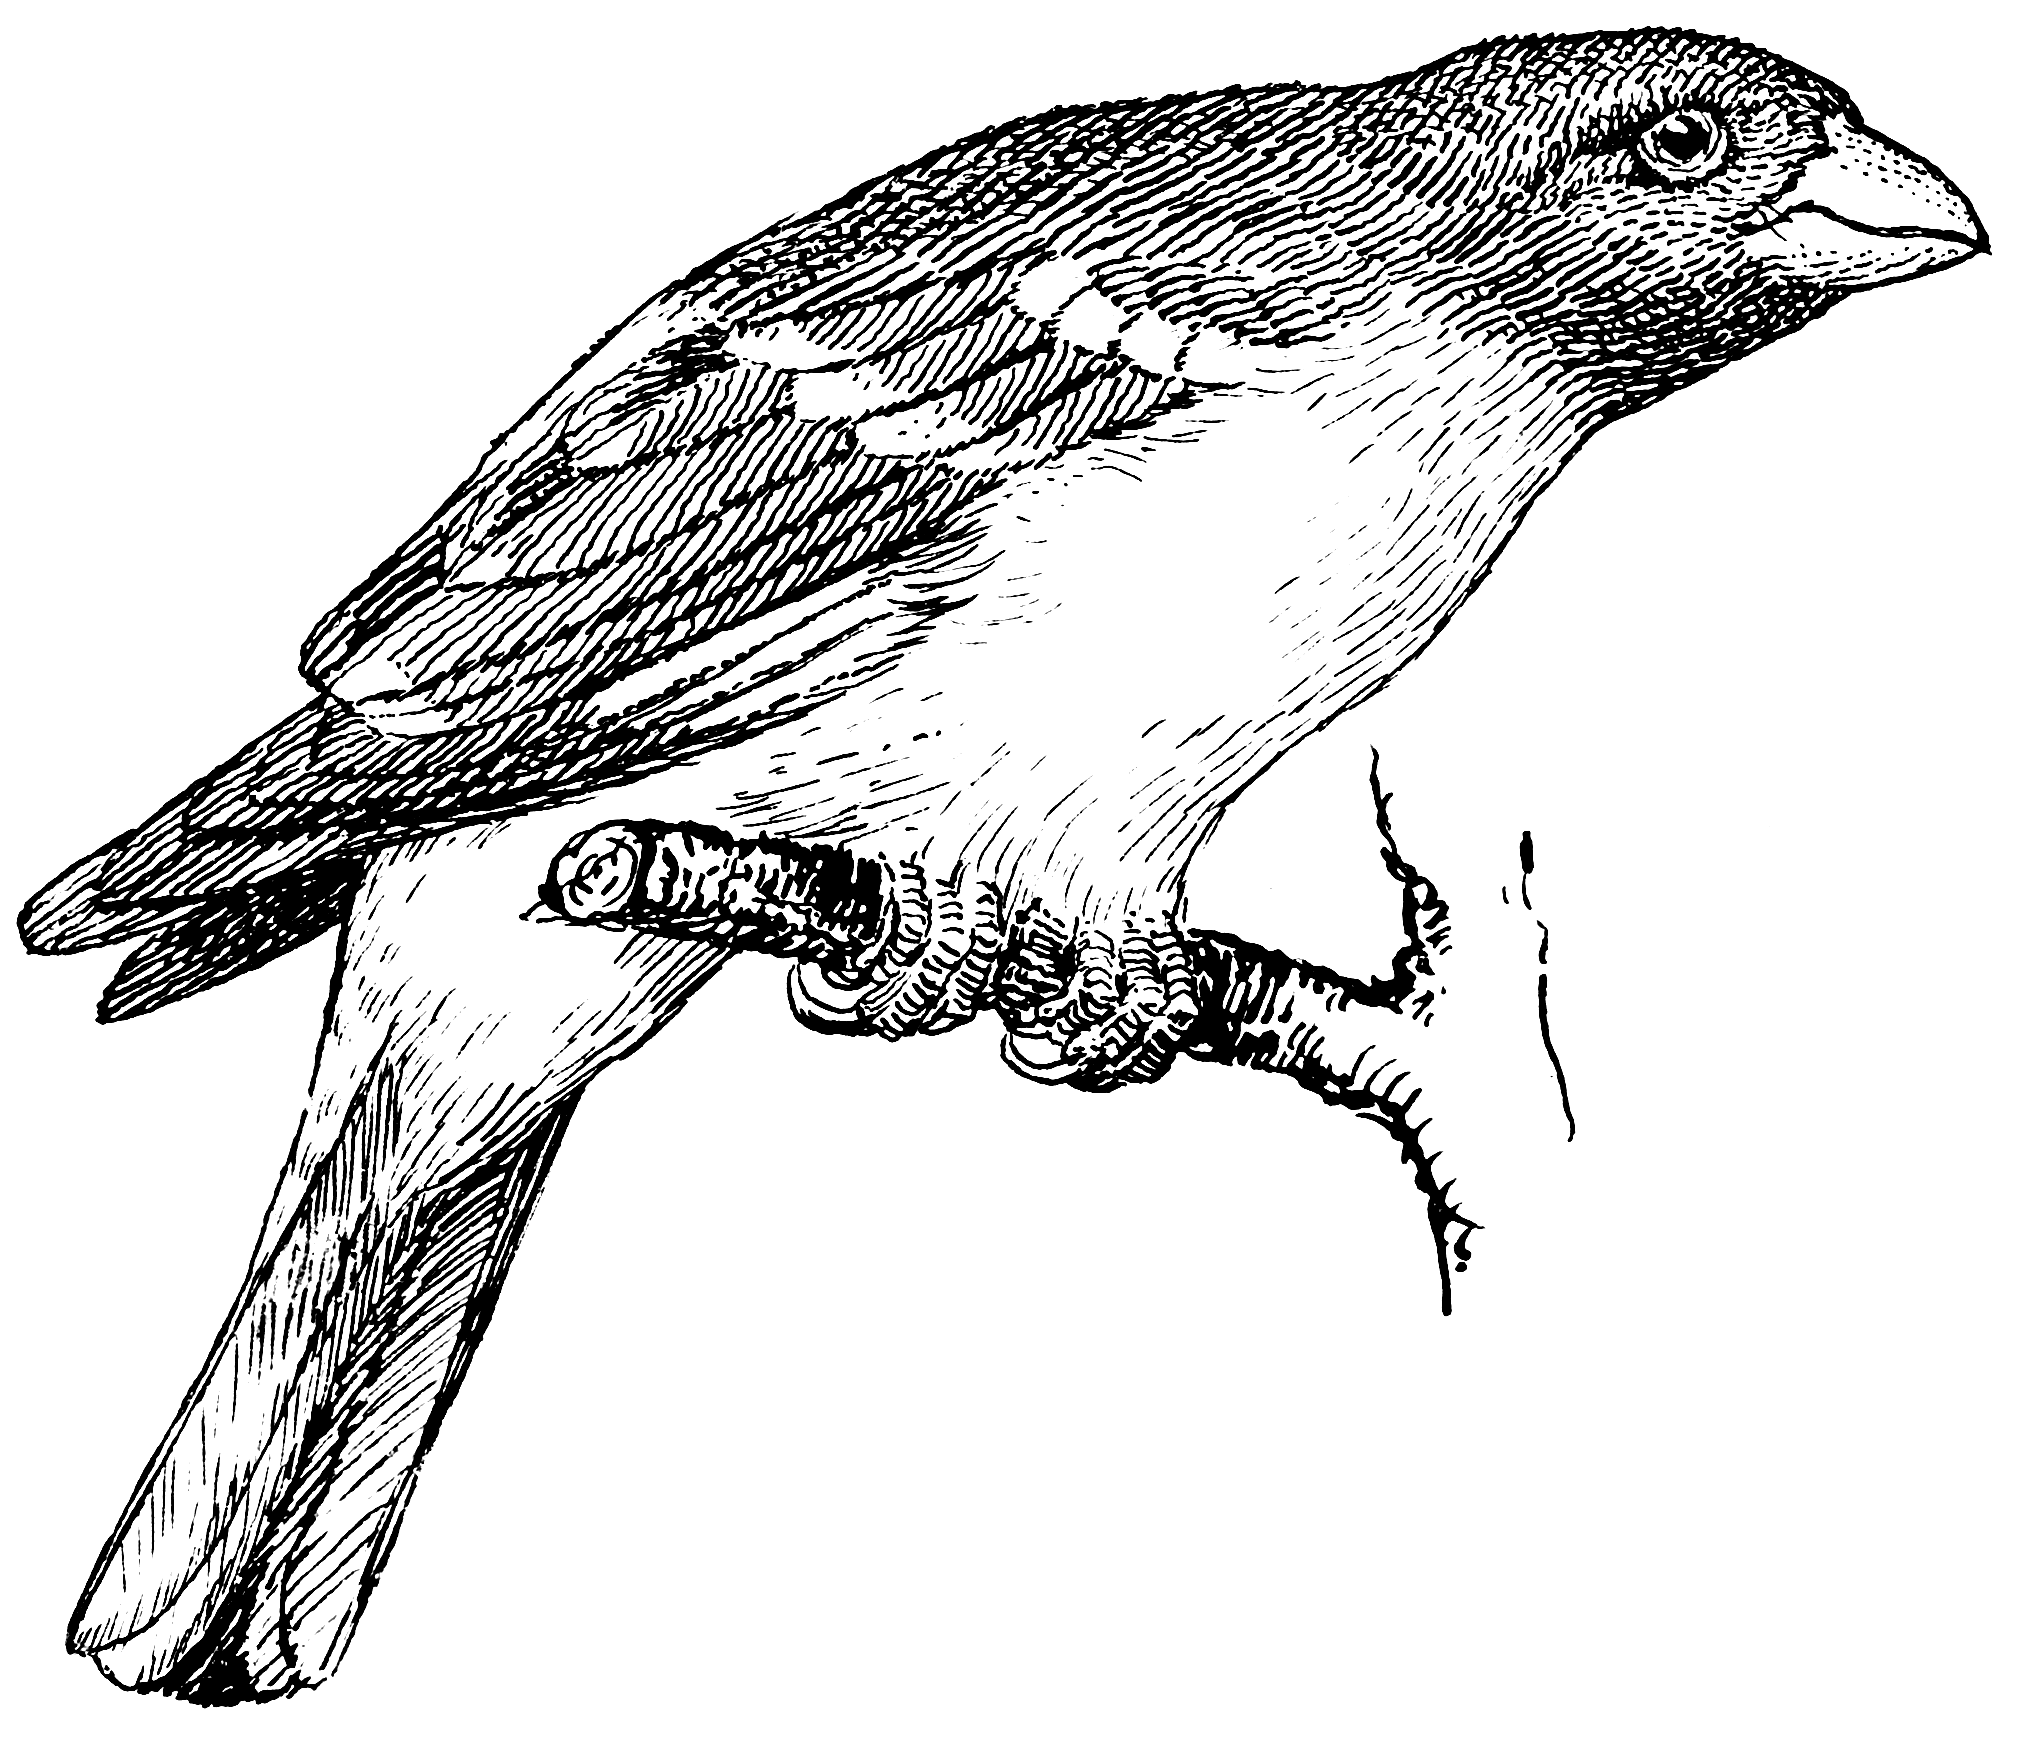
\includegraphics[width=0.5\paperwidth,height=0.5\paperheight,keepaspectratio=true]{img/Grossbeak_(PSF).png}
    \end{wrapfigure}
    \titlepage
  \end{frame}
\end{withoutheadline}

\usebackgroundtemplate{}

%-------------------------------------------------------------------------------

\section{Bird-Song Recognition}
\subsection{In Birdwatching}

\begin{frame}[fragile]
  \vspace{0.5cm}
  {\bfseries\Large In birdwatching}\\
  \vspace{0.5cm}
  \begin{addmargin}{0.5cm}
    \begin{itemize}
      \item Listen for structure and composition:
      \begin{itemize}
        \item Linear tones
        \item Frequency sweeps
        \item Segment repetition
      \end{itemize}
      \item Through auditory perception or sonogram analysis
      \item May encounter difficulties:
      \begin{itemize}
        \item Multiple birds may be singing
        \item Some birds may mimic others
        \item Noisy environment
        \item Too much variety!
      \end{itemize}
    \end{itemize}
  \end{addmargin}
\end{frame}

%-------------------------------------------------------------------------------

\subsection{As a classification problem}

\begin{frame}[fragile]
  \vspace{0.5cm}
  {\bfseries\Large In computing}\\
  \vspace{0.5cm}
  \begin{addmargin}{0.5cm}
    \begin{itemize}
      \item This is a multi-class/multi-label classification problem
      \item Similar problems exist: Vocal recognition, music identification, whalesong classification\ldots
      \item Features are extracted from spectrographic analysis
      \item Machine learning is used to classify the data
      \item We must mitigate the same difficulties:
      \begin{itemize}
        \item Identify multiple, or ignore background species
        \item Distinguish similar birdsongs
        \item Apply noise reduction methods
        \item All across hundreds of recordings
      \end{itemize}
    \end{itemize}
  \end{addmargin}
\end{frame}

%-------------------------------------------------------------------------------

\section{Processing}
%PCM == pulse code modulation
\begin{frame}[fragile]
  \vspace{0.5cm}
  {\bfseries\Large Representing the data}
  \vspace{-0.20cm}
  \begin{figure}
    \includegraphics[clip, trim=0px 320px 0px 20mm, width=1.2\textwidth,center]{img/spec-wav}
  \end{figure}

  \begin{itemize}
    \item A recording is loaded as Pulse Code Modulation (PCM)
   \item We can compute a spectrogram using Short-Time Fourier Transform (STFT)
  \end{itemize}
\end{frame}

\begin{frame}[fragile]
  \vspace{0.5cm}
  {\bfseries\Large Representing the data}
  \vspace{-0.20cm}
  \begin{figure}
    \includegraphics[clip, trim=0px 30px 0px 20mm, width=1.2\textwidth,center]{img/spec-wav}
  \end{figure}
\end{frame}

% In these frames talk about visible shapes and sweeps. maybe we could extract
% information or statistics on the frequency disitrbutions and the audiable
% repetitions? But maybe we have too much noise... leads to next section

%-------------------------------------------------------------------------------

\subsection{Noise Reduction}

\begin{frame}[fragile]
  \vspace{0.5cm}
  {\bfseries\Large Improving SNR}\\
  \vspace{0.5cm}
  \begin{addmargin}{0.5cm}
    \begin{itemize}
      \item Signal to noise ratio might interfere with feature extraction
      \item An \emph{automatic} noise reduction method is requried: \\
        less manual work means more data \& faster iteration
      \item Standard computer vision techniques can be used:
      \begin{itemize}
        \item Median filtering
        \item Thesholding
        \item Dilation \& Erosion
        \item Selective removal of small and/or generic components
      \end{itemize}
    % after a few parameter tweaks we get something more like this...  
    \end{itemize}
  \end{addmargin}
\end{frame}

% Too much noise to run edge detector. Some background noise is not part of the
% signal we are interested in. we want to minimise the SNR.
%
% Automatic noise reduction is necessary to increase the number of samples we
% can use. This is tricky, as noise reduction parameters are not global. We may
% need to automatically fit params to each recording, or make do with a general
% setting, which might be difficult to find.
%
% A combination of computer vision algos can be used
%
% We can apply median filtering for blurring purposes or as a method for
% thresholding, foe example, 1: 3*row,col, 0: otherwise. Blurring the image will
% effectively reduce the contrast of background noise, effectively smoothing it
% out allowing us to threshold it out.
%
% After blurring we can apply binary or limiting threshold to completely remove
% the noise.
%
% Once we have mostly only the important blocks we can dilate and erode in hopes
% of joining contiguous blocks and removing small segments completely.
%
% We can then remove any blocks smaller than a given amount as these usually
% don't belong to the signal we are focusing on, or are too generic to be of
% use.

%-------------------------------------------------------------------------------

\begin{frame}[fragile]
  \vspace{-0.5cm}
  \begin{figure}[!tfp]
    \centering
    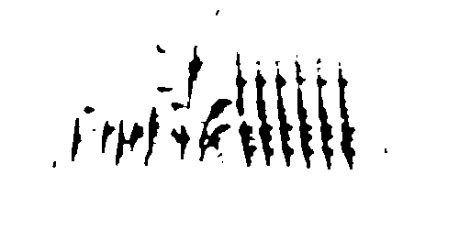
\includegraphics[width=0.8\textwidth]{img/specgram-long-clean}
  \end{figure}

  \vspace{-1cm}

  \begin{addmargin}{0.5cm}
    \begin{itemize}
      \item Global noise reduction parameters is won't work well for every recording
      \item But imperfect results might be close enough through statistical average
      \item Per-recording parameter fitting would be ideal, but more complex
    \end{itemize}
  \end{addmargin}
\end{frame}

% Point out imperfect cleanup. Note that this is impossible w/ global
% parameters, but maybe it doesn't have to be perfect in the first place given
% the quantity of samples that we will have.

%-------------------------------------------------------------------------------

\subsection{Feature Engineering}
\begin{frame}[fragile]
  \vspace{0.5cm}
  {\bfseries\Large Retrieving information}\\
  \begin{figure}
    \includegraphics[clip, trim=0px 1cm 0px 350px, width=1.2\textwidth,center]{img/spec-wav}
  \end{figure}
  \vspace{-0.3cm}
  \begin{addmargin}{0.5cm}
    \begin{itemize}
      \item Dominant frequency domains (pitch)
      \item Characteristic sweeps and tones
      \item Structure:
      \begin{itemize}
        \item repeating components (syllables)
        \item repeating segments
        \item repeating songs
      \end{itemize}
    \end{itemize}
  \end{addmargin}
\end{frame}

%-------------------------------------------------------------------------------

\begin{frame}[fragile]
  \vspace{0.5cm}
  \begin{addmargin}{0.5cm}
    \begin{itemize}
      \item Image recognition can be used\ldots
      \item Components or segments can be cross-correlated against spectrograms
      \item A common approach is template matching:
    \end{itemize}
  \end{addmargin}

    \begin{figure}[!tbp]
      \centering
      \begin{minipage}[c]{0.3\textwidth}
        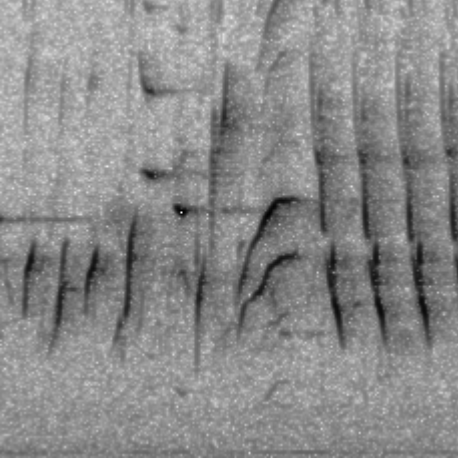
\includegraphics[width=\textwidth]{img/specgram}\\
        {\tiny Raw spectrogram}
      \end{minipage}
      \hfill
      \begin{minipage}[c]{0.3\textwidth}
        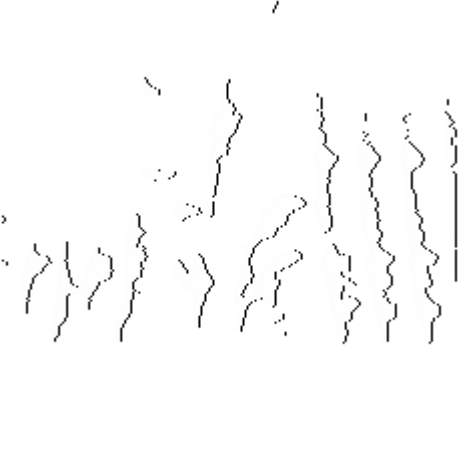
\includegraphics[width=\textwidth]{img/contours}\\
        {\tiny Noise reduction + contours}
      \end{minipage}
      \hfill
      \begin{minipage}[c]{0.3\textwidth}
        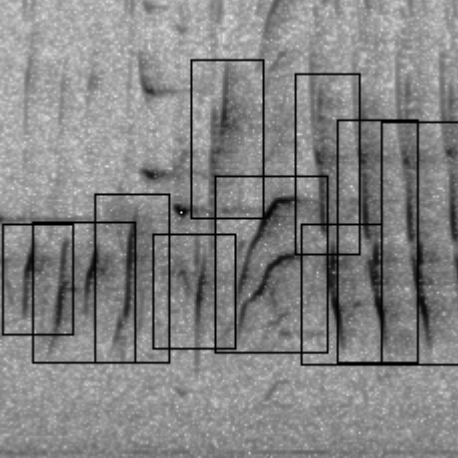
\includegraphics[width=\textwidth]{img/detected-features}\\
        {\tiny Bounding box}
      \end{minipage}
    \end{figure}
\end{frame}

\begin{frame}[fragile]
  \vspace{0.5cm}
  \begin{addmargin}{0.5cm}
    \begin{itemize}
      \item Image recognition can be used\ldots
      \item Components or segments can be cross-correlated against spectrograms
      \item A common approach is template matching:
    \end{itemize}

  \end{addmargin}
    \begin{figure}[!tbp]
      \centering
      \begin{minipage}[c]{0.3\textwidth}
        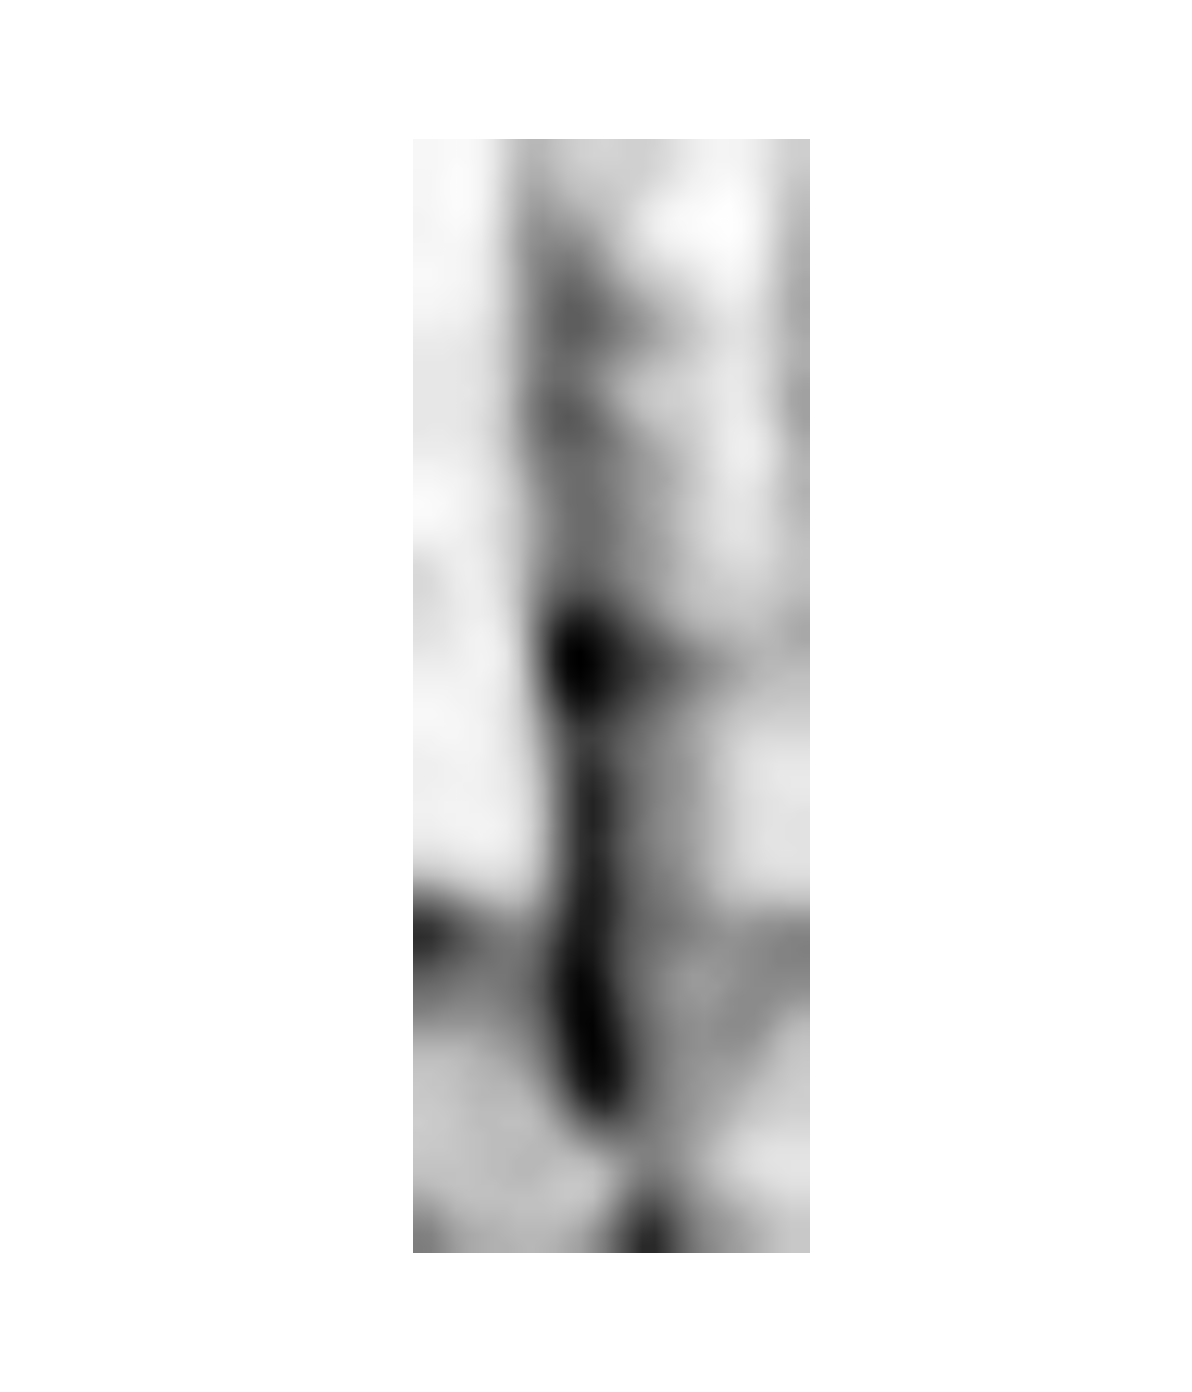
\includegraphics[width=\textwidth]{img/selected-feature}\\
        {\tiny Cropped feature}
      \end{minipage}
      \hfill
      \begin{minipage}[c]{0.3\textwidth}
        \fbox{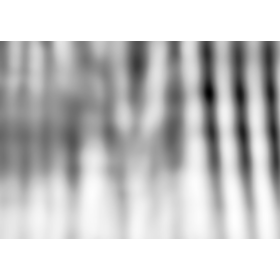
\includegraphics[width=\textwidth]{img/ccm}}\\
        {\tiny Cross-correlation map}
      \end{minipage}
      \hfill
      \begin{minipage}[c]{0.3\textwidth}
        \fbox{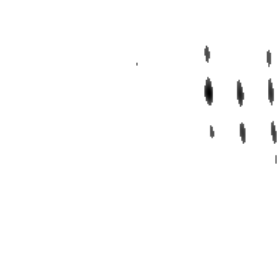
\includegraphics[width=\textwidth]{img/threshold-ccm}}\\
        {\tiny Thresholded CCM}
      \end{minipage}
    \end{figure}
\end{frame}


%-------------------------------------------------------------------------------

\section{Classification}
\subsection{Training}
\begin{frame}[fragile]
  \vspace{0.5cm}
  {\bfseries\Large Classifier training}\\
  \vspace{0.5cm}
  \begin{addmargin}{0.5cm}
    \begin{itemize}
      \item Max-values of cross-correlation mapping results in high dimensional feature vectors
      \item Component and segment detection provides composition statistics, as well as frequency distribution for each species
      \item Many classifiers can be used, but we'll use decision trees (for now)
      \item Multiple, in fact: A random forest of 50--500 trees per class to reduce over-fitting
    \end{itemize}
  \end{addmargin}
\end{frame}

\subsection{Classification}
\begin{frame}[fragile]
  \vspace{0.5cm}
  {\bfseries\Large Classification}
  \vspace{0.5cm}
  \begin{addmargin}{0.5cm}
    \begin{itemize}
      \item Template matching is performed against known templates, producing a similarity feature vector
      \item Statistics are taken from the pre-processed spectrogram
      \item Features are concatenated and fed into each RF
      \item The maximal probability is accepted
      \item Alternatively a probability set is returned
    \end{itemize}
  \end{addmargin}
\end{frame}

\subsection{Accuracy and Performance using AUC}
\begin{frame}[fragile]
  \vspace{0.5cm}
  {\bfseries\Large Classifying accuracy}
  \vspace{0.5cm}
  \begin{columns}[T]
    \begin{column}{0.5\textwidth}
    \begin{itemize}
      \item Accuracy is determined by the area under the Receiver Operating Characteristic curve (AUC)
      \item The cruve represents the resulting TP/FP rate for a given threshold
    \end{itemize}
  \end{column}
  \begin{column}{0.5\textwidth}
    \vspace{-1cm}
    \begin{figure}
      \includegraphics[width=1.0\textwidth]{img/auroc}
    \end{figure}
  \end{column}
  \end{columns}
\end{frame}

% \begin{frame}[fragile] \vspace{0.5cm} {\bfseries\Large Improving performance}
% \vspace{0.5cm} \begin{addmargin}{0.5cm} \begin{itemize} \item High feature
% count and template matching contribute to high computational costs \item
% Discarding less important features should improve accuracy and performance
% \item Template matching can be sped up by blurring templates and target image
% \item We should exploit parallelization and optimizations provided by existing
% libraries \end{itemize} \end{addmargin} \end{frame}


%-------------------------------------------------------------------------------

\section{}
\begin{frame}[fragile]
  \scriptsize
  \begin{figure}
    \def\svgwidth{0.85\columnwidth}
    \input{flow.pdf_tex}
  \end{figure}
\end{frame}

\begin{frame}[fragile]
  \vspace{0.5cm}
  {\bfseries\Large Summary}\\
  \vspace{0.3cm}
    \begin{itemize}
      \item We want to classify several hundred species from field recordings
      \item Noise can interfere with our feature extraction; automatic reduction is necessary
      \item Birdsong can be complex and vary greatly within and across species and regions
      \item Care must be taken to select important features and ignore generic information
      \item Classifier accuracy must be analysed and fed back to tune processing parameters
      \item Immense amounts of data and CV processing can pose computational issues
    \end{itemize}
\end{frame}

\begin{frame}[fragile]
  \nocite{DBLP:conf/mlsp/BriggsHRELCHHBFINTFTNNHRMDVMDCHLM13}
  \nocite{DBLP:conf/mlsp/Fodor13}
  \nocite{DBLP:conf/clef/Lasseck15}
  \nocite{DBLP:conf/clef/Lasseck15a}
  \nocite{DBLP:david_nicholson-proc-scipy-2016}
  \bibliography{bib}
\end{frame}

\end{document}
